\documentclass[acmsmall,nonacm]{acmart}
\settopmatter{printacmref=false,printccs=false}
\graphicspath{{../plots/}}
\begin{document}
\title{Vertex Cover and Greedy Graph Coloring on FRB and Synthetic Graphs}
\author{Ruben Ispiryan}
\authorsaddresses{}
\begin{abstract}
This report compares two vertex-cover algorithms and two greedy graph-coloring orders. The cover algorithms take both ends or one random end of each uncovered edge. The coloring algorithms use the input order or Largest First order. I tested the four implementations on BHOSLIB/FRB graphs and deterministic synthetic graphs. The measurements include runtime and solution size, since a fast method can also give a poor solution. The project includes the code, tests, graph inputs, raw results, and plots.
\end{abstract}
\maketitle

\section{Introduction}
Minimum vertex cover asks for the smallest set of vertices that meets every edge. Graph coloring asks for the fewest colors such that adjacent vertices have different colors. Both optimization problems are hard in general, so simple algorithms are useful when an exact answer is too costly. Assignment 3 specifies the basic edge-pair cover, a randomized one-endpoint version, and basic greedy coloring \cite{assignment}. I compare each pair on the same graph and consider both time and solution quality.

% Confirm that this paragraph reflects your own reasons before submission.
I chose Largest First because I wanted to compare different ways to order vertices for greedy coloring. Basic input order gave me a simple baseline, and Largest First interested me because it uses degree to put more connected vertices first. I wanted to see whether these differences mattered in the measured times and numbers of colors.

\section{Algorithms and Complexity}
Let $V$ be the number of vertices, $E$ the number of undirected edges, and $\Delta$ the maximum degree. The code stores an edge list and adjacency lists, using $O(V+E)$ space. DIMACS parsing and synthetic graph generation are outside the timed algorithm calls. The algorithms use zero-based vertex IDs internally.

\subsection{Basic Vertex Cover}
The basic method scans edges in stored order. If neither endpoint of an edge is already in the cover, it adds both. Later edges incident to either vertex are already covered. This is the assignment's edge-deletion procedure expressed as one pass over the original edges. The selected edges form a maximal matching. If it contains $k$ edges, any cover needs at least $k$ vertices, while this method takes $2k$. It is therefore a 2-approximation \cite{alberta}. With expected constant-time integer set membership, the scan takes $O(E)$ expected time and stores at most $V$ vertices, or $O(V)$ extra space.

\subsection{Randomized Vertex Cover}
The randomized method uses the same edge order, but picks one endpoint of each still-uncovered edge with a seeded local pseudorandom generator. It continues until every edge is covered. Its implementation takes $O(E)$ expected time and $O(V)$ extra space. This exact procedure has no 2-approximation guarantee: on a star, repeated choices of leaves can make the cover much larger than the single center vertex. A seed makes a run reproducible; it does not make the result optimal.

\subsection{Basic Greedy Coloring}
Basic coloring visits vertices in input ID order. It gives each vertex the lowest color not used by an already colored neighbor. One array holds vertex colors and another marks neighbor colors for the current vertex. Each adjacency entry is examined once. Finding a free color checks at most degree$(v)+1$ positions for vertex $v$, so the total is $O(V+E)$ time and $O(V)$ extra space. It always gives a valid coloring and uses at most $\Delta+1$ colors. The actual count depends on the order.

\subsection{Largest First Coloring}
Largest First orders vertices by decreasing \emph{original} degree, breaking ties by vertex ID, then runs the same greedy coloring routine. This is the static order defined by Gebremedhin et al.\ \cite{gebremedhin}; degrees are not changed during ordering. Computing degrees from adjacency lists and sorting vertex IDs takes $O(V+E+V\log V)$ time with this implementation. The coloring pass adds $O(V+E)$, so the full call remains $O(V+E+V\log V)$ time and uses $O(V)$ extra space. Ordering is included in the measured time. The heuristic does not promise fewer colors than input order on every graph.

\begin{table}[t]
\caption{Bounds after the graph representation has been built. Cover set operations have expected constant time.}
\label{tab:complexity}
\centering\small
\begin{tabular}{@{}lll@{}}
\toprule
Method & Time & Extra space \\
\midrule
Basic cover & $O(E)$ expected & $O(V)$ \\
Randomized cover & $O(E)$ expected & $O(V)$ \\
Basic coloring & $O(V+E)$ & $O(V)$ \\
Largest First coloring & $O(V+E+V\log V)$ & $O(V)$ \\
\bottomrule
\end{tabular}
\end{table}

\section{Data and Experimental Method}
The benchmark uses instance 1 from four BHOSLIB/FRB families: 30-15, 35-17, 40-19, and 45-21. The \texttt{.mis} instances are for vertex cover, and the corresponding \texttt{.clq} complement instances are for coloring. The original collection gives the minimum cover size for each MIS graph and the chromatic number for each CLQ graph \cite{bhoslib}. These files have different edge counts. Their optimum values must not be interchanged. All eight input files are included in \texttt{data/frb/}, with checksums in the results metadata.

I also generated sparse graphs with $V=500,1000,2500,5000,10000,20000$ and $E=4V$, plus denser graphs with $V=200,400,800,1200$ and about 10\% of possible edges. The generator uses base seed 520 and a documented derived seed for each graph. It rejects duplicate edges. Each generated graph is reused for both methods of its problem. The cover methods use the same edge order, and the coloring methods start from the same vertex IDs. Synthetic optima are unknown, so no approximation ratio is reported for them.

Each algorithm was timed five times with \texttt{time.perf\_counter\_ns()}. The interval contains only the algorithm call, excluding graph loading or generation, validity checking, CSV output, and plotting. Randomized cover uses seeds 520 through 524. The order of each pair of algorithms rotates across trials to reduce first-run effects. The raw CSV keeps all trials, and the summary CSV gives median time, standard deviation, and solution size. All 280 timed outputs passed an independent validity check after timing. The measurements used Python 3.14.8 on an Apple Silicon macOS laptop. They are Python execution times, not machine-independent operation counts.

\section{Results}
\subsection{Vertex Cover}
Table~\ref{tab:cover} gives the FRB cover results. Both algorithms stayed close to the known minimum on these instances. The randomized method used fewer vertices on two graphs and tied on two, but it was slower in all four cases. Five seeded trials on one instance per family are not enough to claim that it generally gives smaller covers. The basic method has a general 2-approximation guarantee, whereas the randomized version here does not.

\begin{table}[t]
\caption{FRB MIS cover results. Time is median milliseconds and size is the median number of selected vertices.}
\label{tab:cover}
\centering\small
\begin{tabular}{@{}rrrrrrr@{}}
\toprule
$V$ & $E$ & Opt. & Basic ms & Basic size & Random ms & Random size \\
\midrule
450 & 17,827 & 420 & 0.273 & 450 & 0.359 & 449 \\
595 & 27,856 & 560 & 0.465 & 592 & 0.569 & 592 \\
760 & 41,314 & 720 & 0.723 & 760 & 0.856 & 758 \\
945 & 59,186 & 900 & 1.087 & 944 & 1.263 & 944 \\
\bottomrule
\end{tabular}
\end{table}

\begin{figure}[t]
\centering
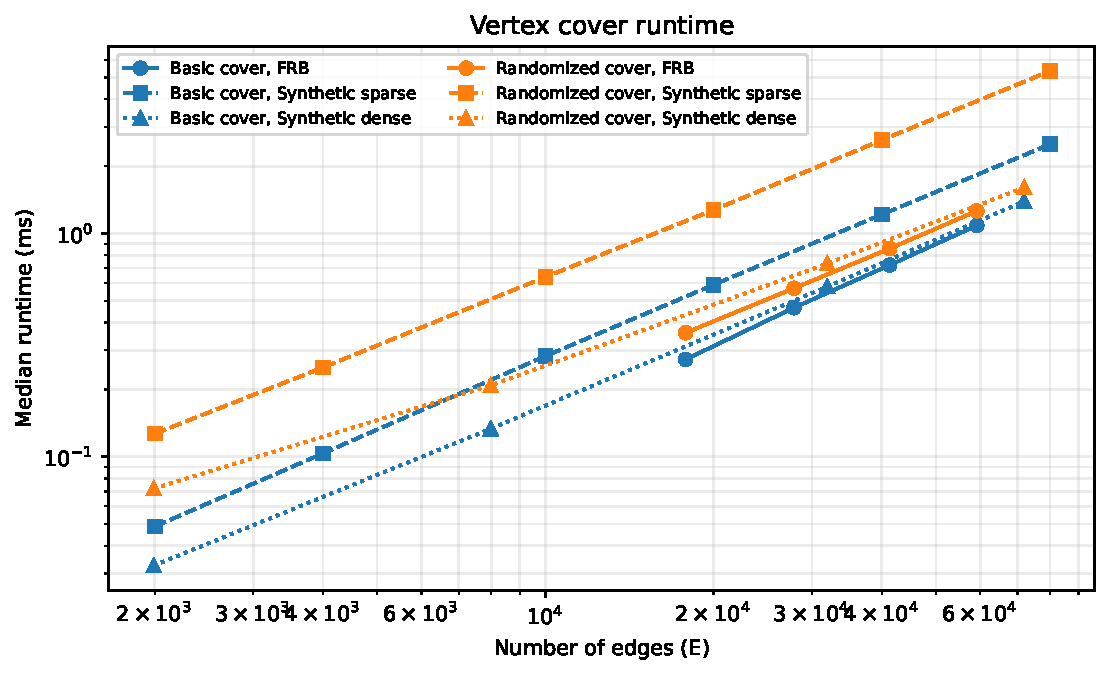
\includegraphics[width=\linewidth]{final_runtime_cover.pdf}
\Description{Logarithmic runtime plot for both cover algorithms on FRB and synthetic graphs.}
\caption{Median cover runtime against edge count. Each point is one measured graph.}
\label{fig:coverruntime}
\end{figure}

Figure~\ref{fig:coverruntime} shows time rising with edge count. Randomized cover does extra random draws and is slower throughout this run. Graphs with similar edge counts can still have different times, because their densities and numbers of uncovered edges differ.

\subsection{Graph Coloring}
Table~\ref{tab:color} gives the FRB coloring results. Basic input order matched the known chromatic number on all four instances. Largest First used more colors, while still producing a valid coloring. This is a real order effect. It shows why Largest First must not be described as always improving greedy coloring. The input numbering of these instances may favor the natural order. This experiment does not establish how the orders compare across all FRB instances.

\begin{table}[t]
\caption{FRB CLQ coloring results. Time is median milliseconds and size is the color count.}
\label{tab:color}
\centering\small
\begin{tabular}{@{}rrrrrrr@{}}
\toprule
$V$ & $E$ & $\chi$ & Basic ms & Basic colors & LF ms & LF colors \\
\midrule
450 & 83,198 & 30 & 2.359 & 30 & 3.033 & 63 \\
595 & 148,859 & 35 & 4.169 & 35 & 5.088 & 63 \\
760 & 247,106 & 40 & 6.888 & 40 & 8.355 & 48 \\
945 & 386,854 & 45 & 10.919 & 45 & 14.152 & 90 \\
\bottomrule
\end{tabular}
\end{table}

\begin{figure}[t]
\centering
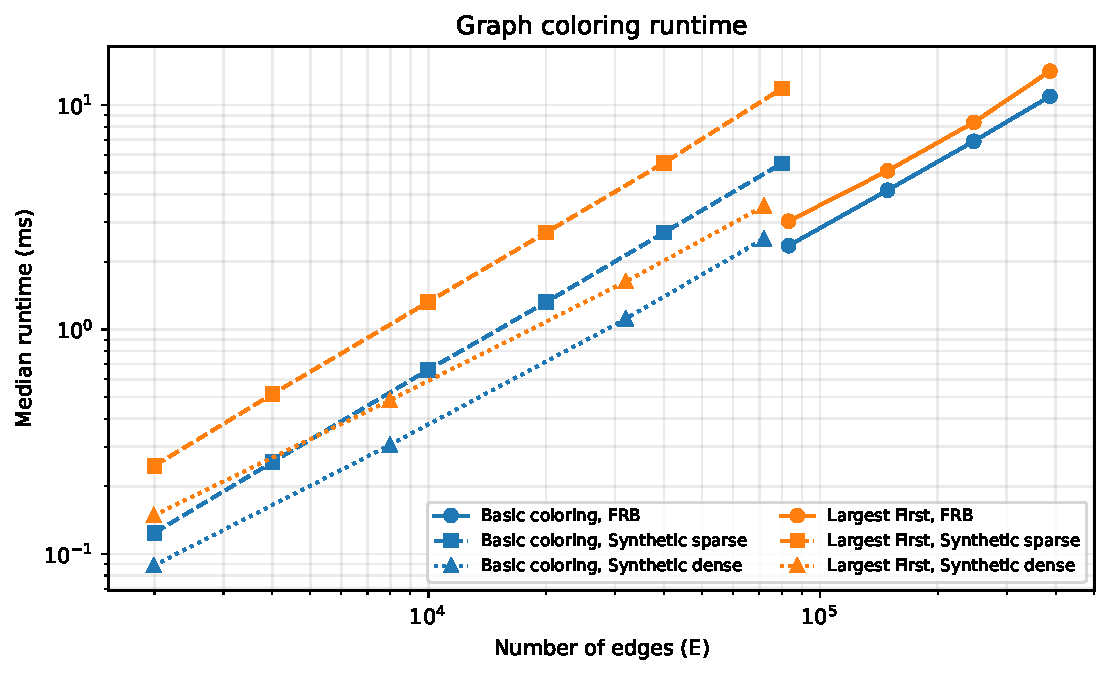
\includegraphics[width=\linewidth]{final_runtime_coloring.pdf}
\Description{Logarithmic runtime plot for basic and Largest First coloring on FRB and synthetic graphs.}
\caption{Median coloring runtime against edge count. Largest First includes sorting time.}
\label{fig:colorruntime}
\end{figure}

Figure~\ref{fig:colorruntime} shows an increasing cost for both methods. Largest First was slower at every measured size. On synthetic graphs, it often saved colors: for the sparse 20,000-vertex graph, basic used 8 and Largest First used 6; for the 1,200-vertex denser graph, they used 36 and 34. The FRB result was the opposite. These cases show how much the order and graph structure matter.

\begin{figure}[t]
\centering
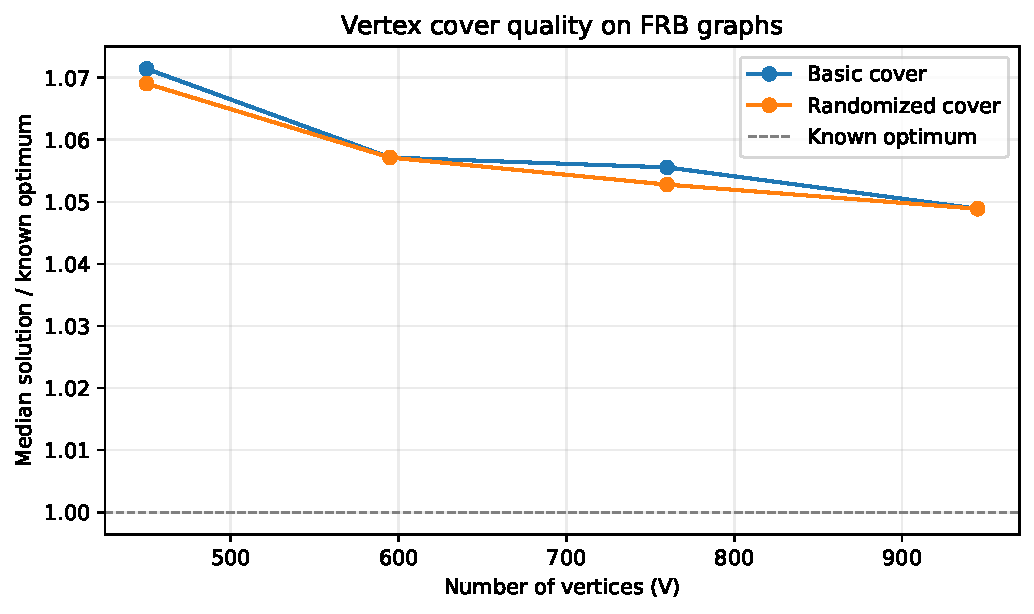
\includegraphics[width=.58\linewidth]{final_quality_cover.pdf}
\Description{Both cover methods return sizes near the known minimum on four FRB MIS instances.}
\caption{Cover size divided by the known minimum on FRB MIS graphs. A ratio of 1 is optimal.}
\label{fig:coverquality}
\end{figure}

\begin{figure}[t]
\centering
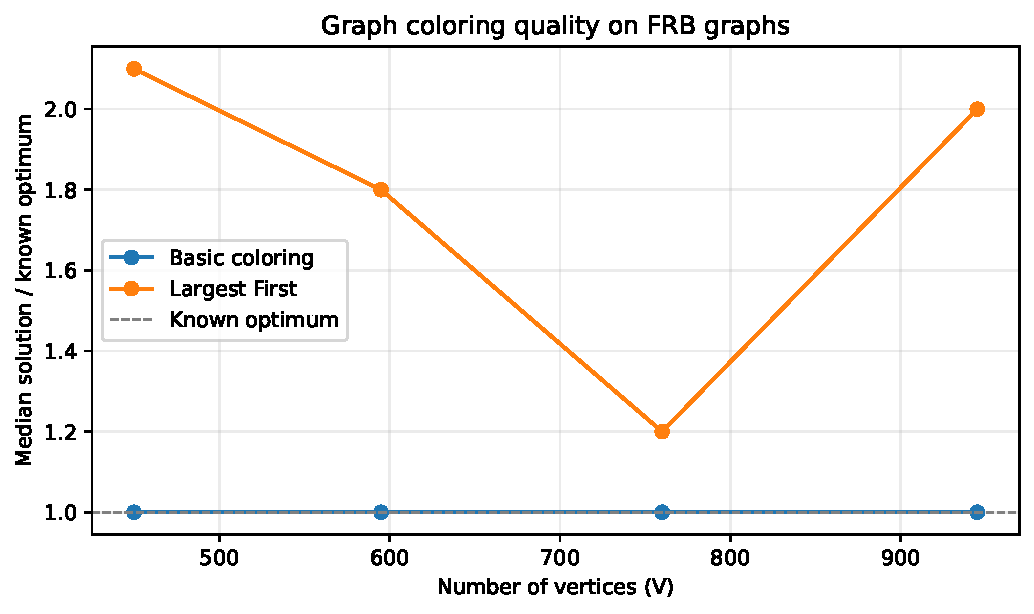
\includegraphics[width=.58\linewidth]{final_quality_coloring.pdf}
\Description{Basic coloring matches the known optimum while Largest First uses more colors on four FRB CLQ instances.}
\caption{Colors used divided by the known chromatic number on FRB CLQ graphs. A ratio of 1 is optimal.}
\label{fig:colorquality}
\end{figure}

Figures~\ref{fig:coverquality} and~\ref{fig:colorquality} show quality relative to each graph's known optimum. The coloring figure is sensitive to the original FRB vertex numbering. More instances and vertex permutations would test whether this difference is typical.

\section{Limitations and Reproduction}
Only one instance from each FRB family is included. The synthetic graphs have exact generation settings but no known optimum. Five seeds give a small sample of the randomized cover's possible results. The cover and coloring runs use different FRB complement files, so cross-problem runtime values should not be read as a direct algorithm comparison. Very short runs can be affected by interpreter and system noise. The raw CSV supports checking the medians and plots.

The implementation and included data are intended for \url{https://github.com/rubenispiryan/cosc520-a3}. The original FRB dataset is at \url{https://rb-bench.github.io/benchmarks/hidden-opt-graph.html}. The repository README gives commands for setup, tests, the demo, benchmarks, plots, and data generation. Unit tests cover validity, the basic cover's bound on small graphs, ordering, parser errors, and deterministic input generation.

\section*{Use of Generative AI}
\begin{itemize}
\item \textbf{OpenAI Codex} assisted with graph generation, benchmark and plotting scripts, unit tests, documentation, README, and report drafting.
\item \textbf{The author} selected Largest First and the graph datasets, wrote the final vertex-cover and graph-coloring implementations, directed and reviewed the work, and takes responsibility for the personal selection reasons in Section 1.
\end{itemize}

\begin{thebibliography}{4}
\bibitem{assignment}
F. H. Fard. 2026. COSC 520 Assignment 3, September 2026. Course handout.
\bibitem{alberta}
University of Alberta. Approximation Algorithms, lecture 1, Section 1.4. \url{https://webdocs.cs.ualberta.ca/~mreza/courses/Approx13/lecture1.pdf}.
\bibitem{gebremedhin}
A. H. Gebremedhin, A. Tarafdar, D. Nguyen, and A. Pothen. 2009. Ordering for Coloring and More. \url{https://eecs.wsu.edu/~assefaw/publications/csc09.pdf}.
\bibitem{bhoslib}
K. Xu. BHOSLIB: Benchmarks with Hidden Optimum Solutions for Graph Problems. \url{https://rb-bench.github.io/benchmarks/hidden-opt-graph.html}.
\end{thebibliography}
\end{document}
